\documentclass[a4paper,12pt]{book} % nie: report!


% pakiety
\usepackage{polski} % lepiej to zamiast babel!
\usepackage[utf8]{inputenc} % w razie kłopotów spróbować: \usepackage[utf8x]{inputenc}
\usepackage{fancyhdr} % nagłówki i stopki
\usepackage{indentfirst} % WAŻNE, MA BYĆ!
\usepackage{lipsum}
\usepackage[pdftex]{graphicx} % to do wstawiania rysunków
\usepackage{amsmath} % to do dodatkowych symboli, przydatne
\usepackage[pdftex,
            left=1in,right=1in,
            top=1in,bottom=1in]{geometry} % marginsy
\usepackage{amssymb} % to też do dodatkowych symboli, też przydatne
\usepackage{pdfpages} % żeby wstawić stronę tytułową
% jesli potrzeb, można oczywiście wstawić inne pakiety i swoje definicje...
 \usepackage{graphicx}
 \graphicspath{{./pictures}}

% definicje nagłówków i stopek
\pagestyle{fancy}
\renewcommand{\chaptermark}[1]{\markboth{#1}{}}
\renewcommand{\sectionmark}[1]{\markright{\thesection\ #1}}
\fancyhf{}
\fancyhead[LE,RO]{\footnotesize\bfseries\thepage}
\fancyhead[LO]{\footnotesize\rightmark}
\fancyhead[RE]{\footnotesize\leftmark}
\renewcommand{\headrulewidth}{0.5pt}
\renewcommand{\footrulewidth}{0pt}
\addtolength{\headheight}{1.5pt}
\fancypagestyle{plain}{\fancyhead{}\cfoot{\footnotesize\bfseries\thepage}\renewcommand{\headrulewidth}{0pt}}

% interlinia
\linespread{1.25}


% treść
\begin{document}
\sloppy



\thispagestyle{empty}

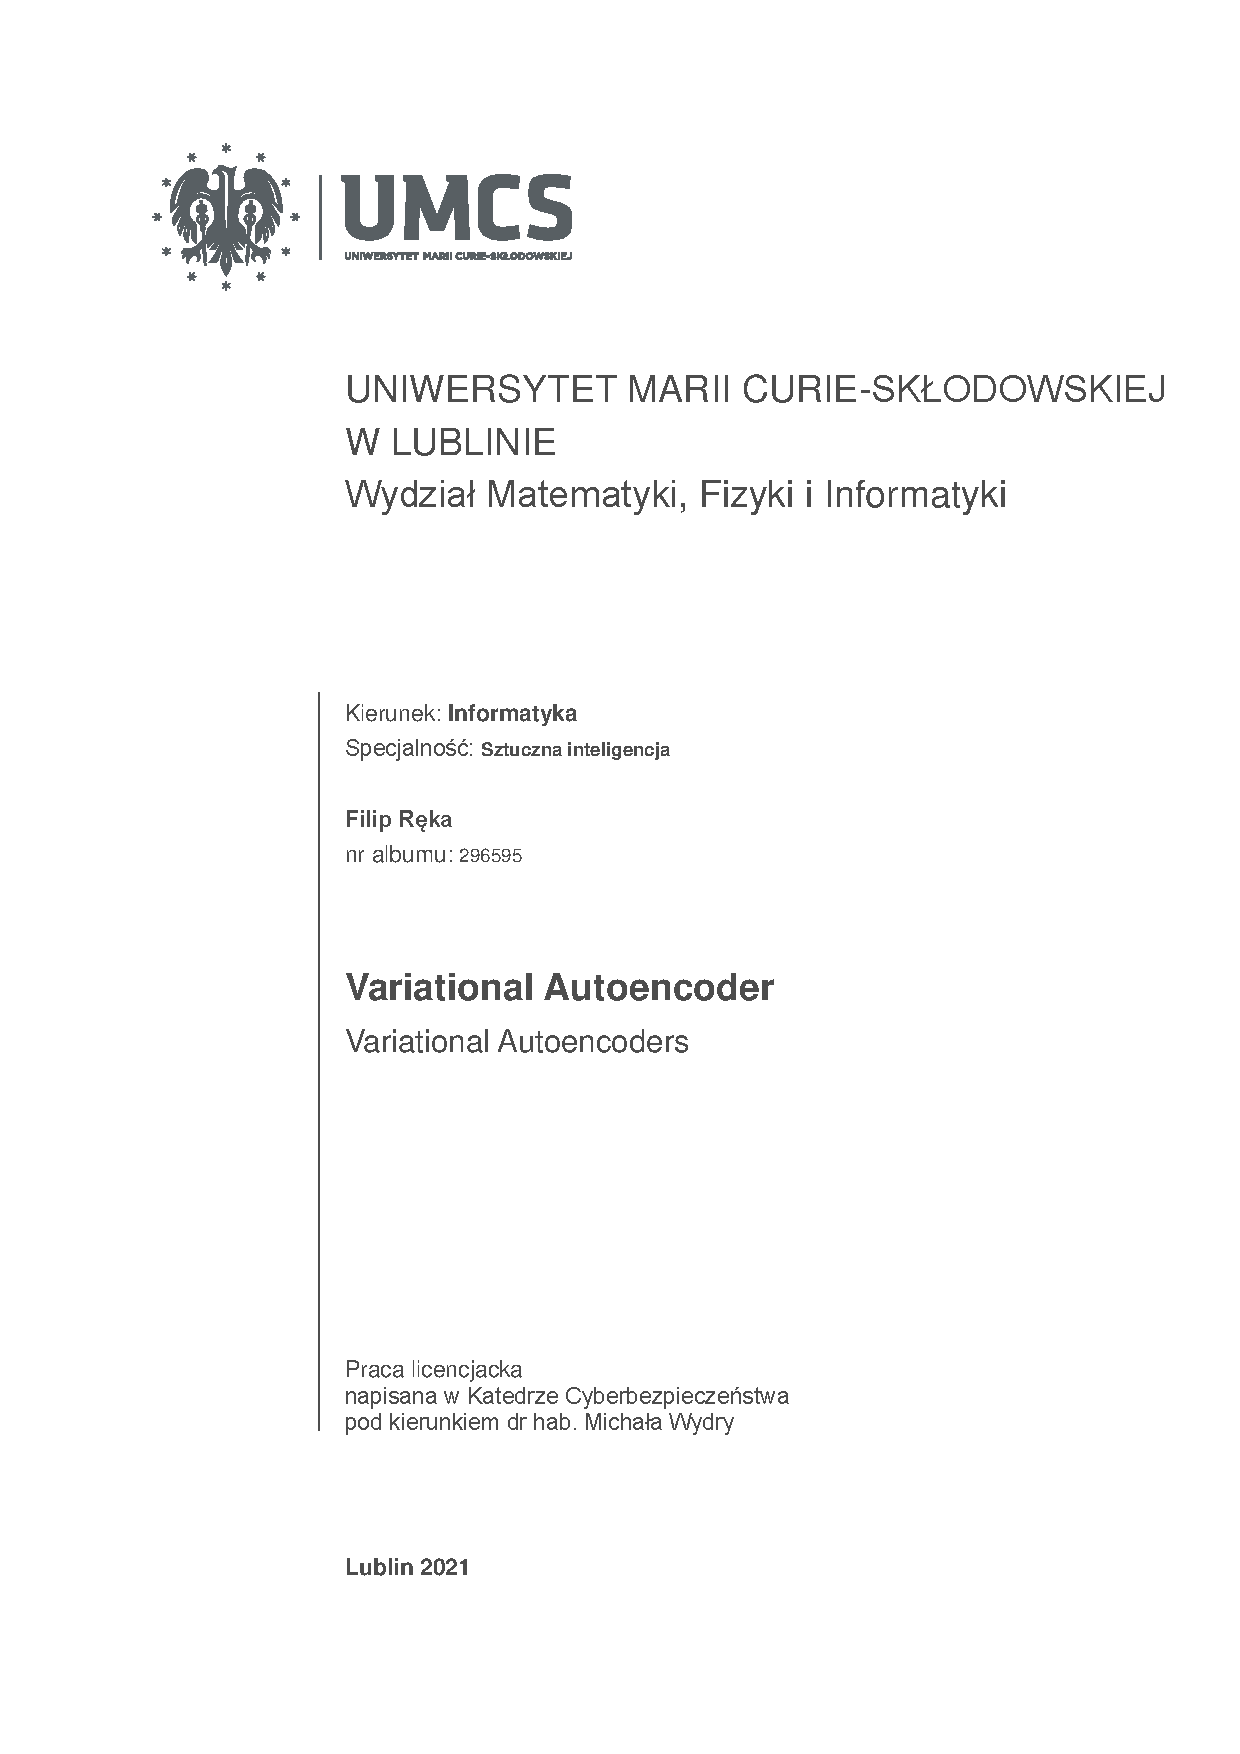
\includepdf{stronatytulowasvg}
% najpierw uzupełnij w 'stronatytulowa.odt' openoffice i wyeksportuj do 'stronatytulowa.pdf'


\thispagestyle{empty}

\tableofcontents{}

\chapter*{Wstęp} % z gwiazdką, więc bez numerka...
\addcontentsline{toc}{chapter}{Wstęp} % ...ale w spisie treści ma być
\textbf{Wariacyjne Autoenkodery} stają się coraz bardziej popularnymi modelami uczenia maszynowego. Zostały zaproponowane przez Diederika P Kingma i Maxa Wellinga. Najczęściej zostają one skategoryzowane do modeli uczenia częściowo nadzorowanego. Znajdują zastosowanie w generacji obrazów, tekstu, muzyki, odszumianiu obrazków, sygnałów oraz w detekcji anomalii. W przeciwieństwie do tradycyjnych autoenkoderów prezentują pobabilistyczne podejście do generowania zmiennych ukrytych. Swoją popularność zawdzięcza swojej budowie, która jest oparta na sieciach neuronowych oraz możliwości trenowania go przy pomocy metod gradientowych.
\chapter{Tradycyjny autoenkoder} 
\section{Informacje wstępne}
Autoenkoder jest specyficzną wersją sieci neuronowej składającej się z dwóch części: enkodera, który koduje dane wejściowe oraz dekodera, który na podstawie kodu rekonstruuje wejście.\cite{bank2021autoencoders} Architektura enkodera wymaga aby jego warstwa wyjściowa generująca reprezentacje danych była mniejsza niż warstwa wejściowa. Często zwężenie jest nazywane \textit{bottle neck}. Model na swoją warstwę wejściową oraz wyjściową dostaję te same dane. Celem treningu całego autoenkodera jest zminimalizowanie błędu pomiędzy prawdziwymi danymi wejściowymi, a tymi odkodowanymi ze skompresowanych wartości. W przypadku obrazów funkcją straty może być na przykład błąd średniokwadratowy, który powie nam, jak wynik różni się od wejścia. \\
Powiedzmy że mamy dane wejściowe $X$ o wymiarze $m$ oraz chcemy je zakodować do wymiaru $n$. Formalnie możemy zapisać, że model próbuje nauczyć się funkcji:
\begin{center}
	Enkoder $E : \mathbb{R}^m \rightarrow \mathbb{R}^n$\\
	Dekoder $D: \mathbb{R}^n \rightarrow \mathbb{R}^m$ \\
	gdzie $n < m$\\
	$\mathcal{L}(x, \hat{x}) = \dfrac{1}{m}\displaystyle\sum_{i=0}^{m}(x_i-\hat{x}_i)^2 = \dfrac{1}{m}\displaystyle\sum_{i=0}^{m}(x_i-D(E(x_i)))^2$
\end{center}
Calem \textit{bottle neck-a} jest skompresowanie wejścia i zachowanie w ukrytych wartościach jak najwięcej informacji. W momencie, kiedy $n = m$ model przekazałby wartości z pierwszej warstwy na ostatnią bez potrzeby kompresji.

\begin{figure}[h]
	\centering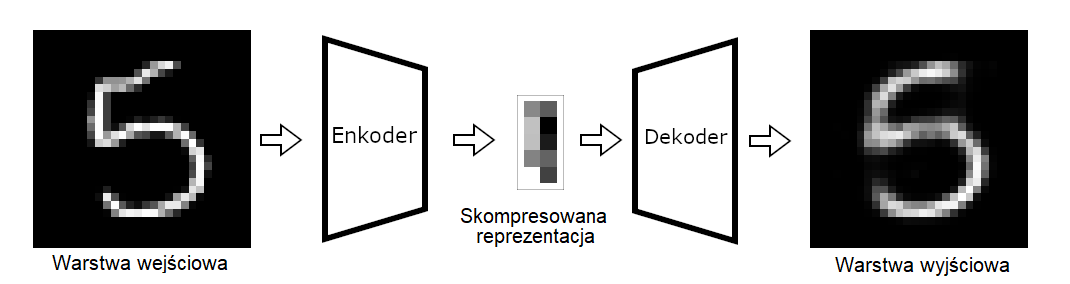
\includegraphics[width=14.5cm]{pictures/autoencoder.png}
	\caption{Obrazek jest zakodowany do skompresowanej reprezentacji, a następnie zostaje odkodowany przez dekoder.}
\end{figure}
\section{Zastosowania}
\subsection{Redukcja wymiarów}
\lipsum[1]
\subsection{Odszumianie obrazów}
\lipsum[2]
\begin{figure}[h]
	\centering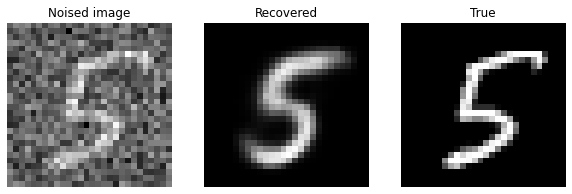
\includegraphics[width=14.5cm]{pictures/noised1.png}
	\caption{Grafika przedstawia porównanie obrazu z szumem, prawdziwego oraz wynikowego odkodowanego z czterech wartości.}
\end{figure}
\subsection{Uzupełnianie obrazów}
\lipsum[1-2]
\begin{figure}[h]
	\centering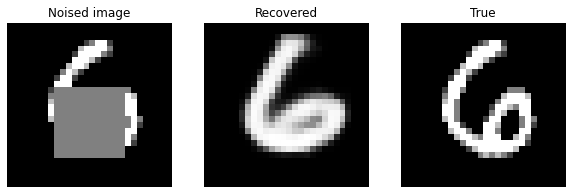
\includegraphics[width=14.5cm]{pictures/completion1.png}
	\caption{Grafika przedstawia porównanie obrazu wejściowego, prawdziwego oraz wynikowego odkodowanego z czterech wartości.}
\end{figure}

\section{Problemy z generacją nowych danych}
Dobrym pytaniem jest czy przy pomocy kodu jesteśmy generować nowe dane bardzo podobne do tych co model otrzymał na wejściu. Wytrenowaliśmy sieć, która jest w stanie ze zmiennych ukrytych odkodować obraz, więc ustawiając wejście dekodera na losowy punkt z przestrzeni zmiennych powinniśmy być w stanie dostać obraz, który jest podobny do tych na których sieć została wytrenowana.
Aby model mógł generować nowe dane muszą zostać spełnione dwa warunki:
\begin{itemize}
	\item Nasza przestrzeń kodu (tzw. zmiennych ukrytych) musi być ciągła co znaczy że dwa punkty znajdujące się obok siebie będą dawać podobne dane jak zostaną odkodowane
	\item Przestrzeń musi być kompletna co znaczy, ze punkty wzięte z dystrybucji muszą dawaj wyniki mające sens
\end{itemize}
Tradycyjna architektura nie zapewnia nam a priori czy przestrzeń zmiennych ukrytych będzie spełniała te warunki. Zadaniem modelu jest jak najlepsze odzwierciedlenie skompresowanych danych, a nie dbanie o to, czy rozkład zmiennych kodu spełnia nasze warunki. Może się tak zdarzyć, że siec nauczy się akurat takiej dystrybucji, która by nam pasowała, ale jest to bardzo mało prawdopodobne. Jeśli chcemy zbudować model generacyjny musimy mieć zagwarantowane, że za każdym razem dostaniemy rozkład spełniający nasze warunki. 
\chapter{Wariacyjny autoenkoder}
\section{Informacje ogóle}
Wariacyjny autoenkoder ma inne podejście do generowania zmiennych ukrytych. Zamiast generować jedną zmienną dla każdego wymiaru, generuje dwie liczby, $\sigma$ oraz $\mu$, które traktujemy jako odchylenie standardowe oraz średnią rozkładu normalnego.
Dla przykładu jeśli uznamy ze chcemy dane reprezentować jako siedmio-wymiarowy wektor, nasz enkoder wygeneruje dwa wektory siedmio-wymiarowe, z którego jeden będzie przechowywał wartości średniej a drugi odchylenia standardowego dla każdego z siedmiu rozkładu normalnego. Kolejną istotną zmiana jest funkcja straty, która oprócz błędu rekonstrukcji obrazu składa się z dywergencji Kullbacka-Leiblera.\\
\section{Motywacja statystyczna}
Powiedzmy ze istnieje zmienna ukryta $z$, która generuje obserwację $x$. Mamy tylko informację o $x$ i chcemy się dowiedzieć jakiej jest $z$. Aby to zrobić powinniśmy policzyć $p(z|x)$. Z twierdzenia Bayesa wiemy że:\\
\begin{center}
	$p(z|x)=\dfrac{p(x|z)p(z)}{p(x)}$
\end{center}
Aby obliczyć rozkład marginalny $p(x)$ musimy policzyć:
\begin{center}
	$p(x) = \displaystyle\int_{z}^{}p(x,z)dz$
\end{center}
Obliczenie tej całki jest bardzo trudne ponieważ $z$ jest często wielowymiarowe i przestrzeń przeszukiwań jest zwyczajnie kombinatorycznie za duża aby korzystać z takich metod jak próbkowanie Monte Carlo łańcuchami Markowa. \\

\section{Wnioskowanie wariacyjne}
Rozwiązaniem tego problemu jest próba policzenia rozkładu $q(z|x)$, które będzie jak najlepiej odzwierciedlać $p(z|x)$ i będzie miał rozkład, który będziemy mogli policzyć. 
\subsection{Dywergencji Kullbacka-Leiblera}
Jest to miara określająca rozbieżność między dwoma rozkładami prawdopodobieństwa. Nie można określić jej mianem metryki ponieważ nie jest symetryczna ($D_{KL}(P\|Q)\neq  D_{KL}(Q\|P)$).\\ Naszym celem będzie zminimalizowanie jej.
\begin{center}
	$q^\ast(z|x)=\operatorname*{argmin}_{q(z|x)\in Q}(D_{KL}(q(z|x)\|p(z|x)))$
	\\gdzie $Q$ to rodzina prostych dystrybucji, na przykład rozkładu Gaussa 
\end{center}
Policzmy:
\begin{center}
	$D_{KL}(q(z|x)\|p(z|x))=\mathbb{E}_{z\sim q(z|x)}\log\dfrac{p(z|x)}{q(z|x)} = 
	\displaystyle\int_{z}^{}q(z|x)\log\frac{q(z|x)}{p(z|x)}dz$
\end{center}
	 Natrafiamy na kolejny problem ponieważ nie możemy $p(z|x)$ jednak jesteśmy w stanie to przepisać jako:\\
\begin{center}
	$p(z|x)=\dfrac{p(z,x)}{p(x)}$
\end{center}
Tu jest dużo matmy której nie chce mi się na razie pisać ale tu będzie ELBO (dolna granica dowodów).
\newpage
Wybieramy sobie że nasza funkcja $q(z|x)$ będzie $\mathcal{N}(0, \textit{\textbf{I}})$.
Dywergencja dla dwóch rozkładów normalnych wygląda w następujący sposób. 
\begin{center}
	$\dfrac{1}{2}\left\{\left(\dfrac{\sigma_0}{\sigma_1}\right)^2+\dfrac{(\mu_1 - \mu_0)^2}{\sigma_1^2} - 1 + 2\log\dfrac{\sigma_1}{\sigma_0}\right\}$
\end{center}
Co w naszym przypadku gdzie $\mu_1 = 0$ oraz $\sigma_1=1$ uprości się do:
\begin{center}
	$\dfrac{1}{2}\displaystyle\sum_{m}^{i=1}\sigma_i^2+\mu_i^2-2\log(\sigma_i)-1$
\end{center} 
Jest to pierwsza część naszej funkcji straty. 
\newpage
\section{Sztuczka reparametryzacyjna}
Model \textit{VAE} po zakodowaniu wejścia dokonuje operacji próbkowania (\textit{sampling}) z dystrybucji na nauczonych parametrach. Przy propagacji do przodu nie jest to problem, jednak podczas propagacji wstecznej jest to nie możliwe. Operacja próbkowania nie jest różniczkowalna co sprawia, że nie możemy policzyć gradientu. Sposobem obejścia tego problemu jest zastosowanie sztuczki (\textit{reparameterization trick}). Próbkowanie z dystrybucji $z\sim\mathcal{N}(\mu, \sigma)$ jesteśmy w stanie zapisać jako:
\begin{center}
	$\epsilon\sim\mathcal{N}(0,1)$\\
	$z=\mu+\sigma\bigodot\epsilon$
\end{center} 
Pozornie nic się nie zmieniło, jednak teraz jesteśmy w stanie poprowadzić gradient przez $z$, które jest teraz deterministycznie. W poprzednim przypadku było ono losowe wybierane z dystrybucji. 

\chapter{Implementacja}
\section{Tensorflow oraz Keras}
\lipsum[1]\cite{doersch2021tutorial}

\listoftables{} % jeśli są tabele
\addcontentsline{toc}{chapter}{Spis tabel}

\listoffigures{} % jeśli są tabele
\addcontentsline{toc}{chapter}{Spis rysunków}

\bibliographystyle{ieeetr}
\bibliography{./cytowania/cytowania.bib}

\end{document}
